
\chapter{Case Study}
\label{chapter4}

\graphicspath{{Chapter4/figs/}}

This chapter focuses on discussing about a possible analysis path with MLExplore.js for one real-world dataset. In general terms, this path consist of two stages: (1) Load the dataset and perform a first overview for gaining a general understanding about this, (2) iteratively navigate the data and perform attribute selection and train multiple t-SNE and K-Means models for identifying local and global structural changes (cluster formation) in the data, and (3) explain the results in terms of the original attributes by observing their distribution among clusters or predefined classes and selecting some data instances of interest for perform neighbors analysis.

The SALURBAL dataset is introduced in \ref{section1.1}. An additional detail about this dataset is the complexity of the attributes reflecting Urban Landscape, Street Design and Transportation domains for the 1.433 Latin American sub-cities included in the study. Researchers currently have used Finite Mixture Models for the Urban Landscape and Street Design domains to determine profiles emerging from the sub-cities. The first challenge consist of determining the set of hyper-parameters that enables the identification of representative profiles based on entropy and Bayesian Information Criterion. The second challenge is about determining differences among profiles and naming them.

Figure \ref{fig:salurbal-case-study-1} shows MLExplore.js after the user loads the SALURBAL dataset and by default a t-SNE model is trained using all numerical attributes. Thanks to Navio, it is possible to evidence that many attributes are highly correlated and some others have a high missing value ratio. TRANS\_PROF is the categorical attribute automatically selected for color encoding. This attribute represents the Street Design profile previously obtained using the Finite Mixture Models. User can also use URBAN\_PROF (Urban Landscape profile) for color encoding selecting this attribute in the upper-right combobox of the Attribute Selection component.

\begin{figure}[ht]
 \centering
 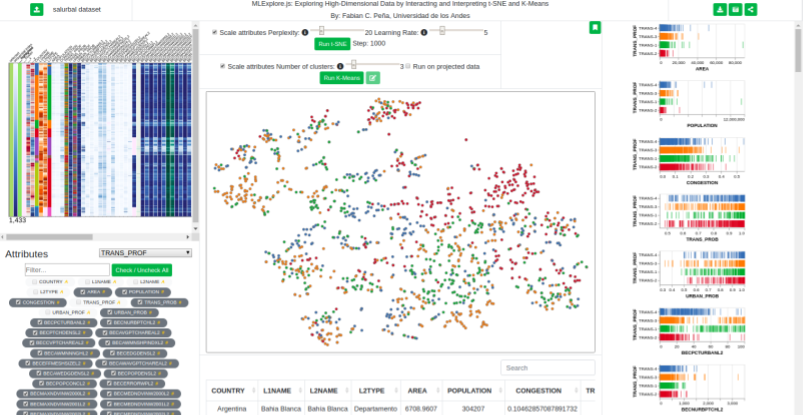
\includegraphics[width=0.9\textwidth]{salurbal-case-study-1.png}
 \caption{First iteration in MLExplore.js for the SALURBAL dataset.}
 \label{fig:salurbal-case-study-1}
\end{figure}

For both domains, just a subset of attribute are selected for training the models: Street density, Intersection density, Streets per node average, Street length average and circuity average, for Street Density, and Number of urban patches, Patch density, Area-weighted mean patch size, Effective mesh size, Area-weighted mean shape index and Area-weighted mean nearest neighbor distance, for Urban Landscape. MLExplore.js is updated for including in each case only these attributes and training again the t-SNE models with the same hyper-parameters: 20 for perplexity and 5 for learning rate. Figure \ref{fig:salurbal-case-study-2} evidences the embedding results for this interaction with the Attribute Selection component.

\begin{figure}[ht]
 \centering
 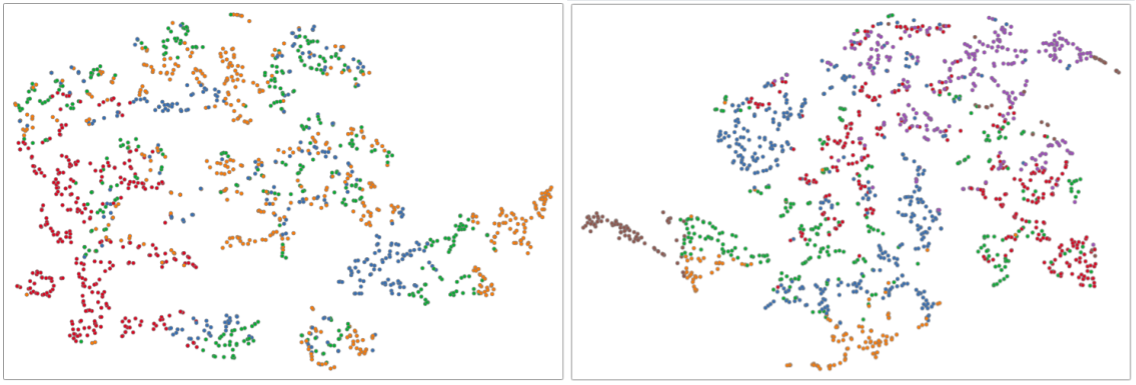
\includegraphics[width=1.0\textwidth]{salurbal-case-study-2.png}
 \caption{t-SNE for Street Design (left) and Urban Landscape (right) selected attributes.}
 \label{fig:salurbal-case-study-2}
\end{figure}

Because the visually identified clusters for both domains seems to be so granularized, dominating local data structure, perplexity t-SNE hyper-parameter can be increased to obtain a more compact group. According to Figure \ref{fig:salurbal-case-study-3}, for perplexity equal to 50, the resulting embedding is able to locate instances of the same cluster near, as the case of the red cluster in the Street Design embedding (left) and the brown cluster in the Urban Landscape embedding (right). Reasons behind the difficulty of finding an embedding that better reflects the profiles could be that Finite Mixture Models and t-SNE optimize in a different way and the same domain complexity. While Finite Mixture Models is a probabilistic model, t-SNE learns from similarity metrics such as euclidean distance. Maybe, K-Means could works better with the t-SNE for producing clusters that can be visually identified in a more clear way.  

\begin{figure}[ht]
 \centering
 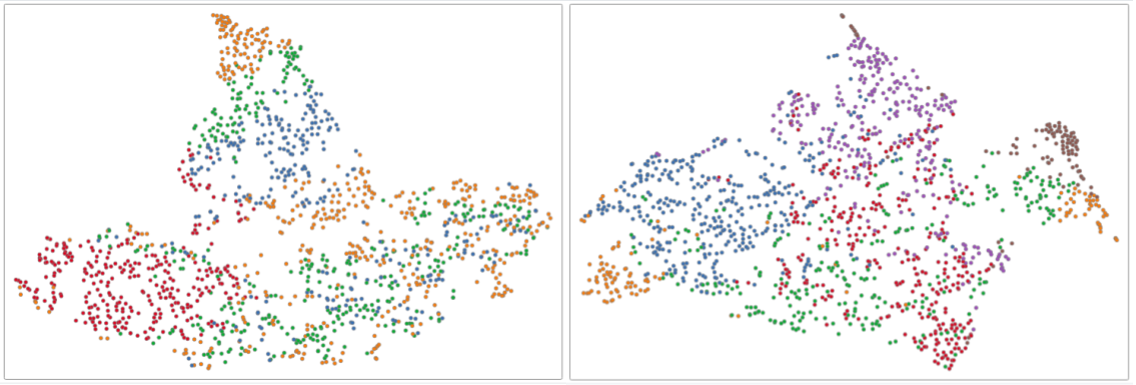
\includegraphics[width=1.0\textwidth]{salurbal-case-study-3.png}
 \caption{t-SNE for Street Design (left) and Urban Landscape (right) selected attributes when increasing perplexity to 50.}
 \label{fig:salurbal-case-study-3}
\end{figure}

Two new t-SNE and K-Means models for Street Design and Urban Landscape domains are trained. Figure \ref{fig:salurbal-case-study-4} shows the result for the Street Design profile where K-Means clusters are better identified in the t-SNE embedding with less cluster overlapping in comparison with profiles from the Finite Mixture Models. In Attribute Distribution component is possible to observe that the cluster orange characterizes by high values of Street density while the cluster green by high values in Intersection density and Streets per node average. Unfortunately, K-Means evidences some limitations when instances have outlier values tending to create an independent cluster for that few instances. In this case, Colon, Panama, having a very high Circuity average. Urban Landscape domain, Figure \ref{fig:salurbal-case-study-5}, have a similar problem creating two clusters with very few sub-units.

\begin{figure}[ht]
 \centering
 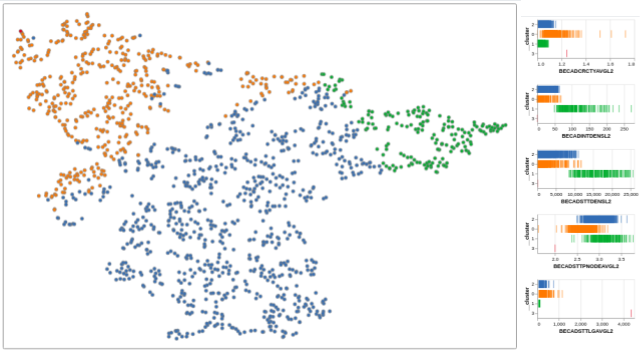
\includegraphics[width=0.8\textwidth]{salurbal-case-study-4.png}
 \caption{t-SNE and K-Means for Street Design selected attributes and clustering results in the Attribute Distribution panel.}
 \label{fig:salurbal-case-study-4}
\end{figure}

\begin{figure}[ht]
 \centering
 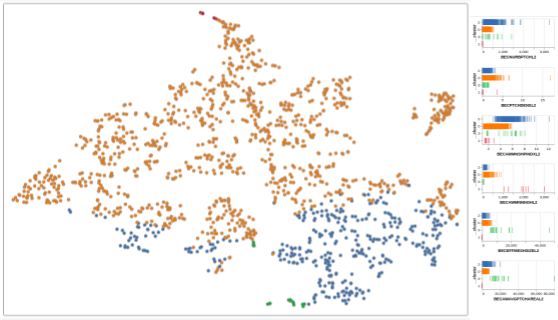
\includegraphics[width=0.8\textwidth]{salurbal-case-study-5.png}
 \caption{t-SNE and K-Means for Urban Landscape selected attributes and clustering results in the Attribute Distribution panel.}
 \label{fig:salurbal-case-study-5}
\end{figure}